\chapter{Introduction}

\vspace{-1em}

When we observe the sky, we perceive it as a 2D surface, even though celestial objects actually exist in 3D space. To bridge this gap and measure distances in astronomy it is used a set of techniques known as the \textit{distance ladder}. It consists of different methods, where each one relies on a specific physical phenomenon and is calibrated using the preceding method in the ladder. Only recently have precise instruments like ESA's Hipparcos (1989) and Gaia (2013) satellites enabled highly accurate stellar parallax measurements, with Gaia mapping distances to over a billion stars.

\vspace{-0.5em}

\section{Reference Systems}

To describe the position of an object in the sky, we need to define a reference system. For this purpose, astronomers often imagine all celestial objects as lying on a vast, imaginary \textit{celestial sphere}, centered on the observer. Although this model has ancient origins, it remains extremely useful today. Since the celestial sphere is considered to have an infinite radius, we can ignore the small shifts caused by the Earth's rotation and orbit.

   \subsection{The Equatorial System}

The \textbf{equatorial system} is defined by selecting a reference parallel and a reference meridian. The Earth's rotational axis remains nearly constant over time, so the equatorial plane (which is perpendicular to this axis) serves as a stable basis for a coordinate system that does not depend on the observer’s location or the time of observation.

The \bfit{celestial equator} is the great circle where the celestial sphere meets the equatorial plane. The axis of this circle points toward the celestial poles. In the northern hemisphere, the north celestial pole is almost exactly aligned with the Earth's rotational axis and lies about one degree from Polaris.

\vspace{0.2em}

\begin{minipage}{0.55\textwidth}
    The angle between a star and the celestial equator (the equatorial plane) remains unchanged by the Earth's daily rotation. This angle is called the \bfit{declination} $\delta$ ($-90^\circ < \delta < +90^\circ$).
    For the second coordinate, we also need a fixed direction that is independent of the Earth's rotation. This direction is defined by the \textit{vernal equinox} (\Aries), which is the point on the celestial sphere where the Sun's path (the ecliptic) crosses the celestial equator at the moment of the spring equinox. The second coordinate is then defined as the angle measured eastward along the celestial equator from the vernal equinox. This angle is called the \bfit{right ascension} $\alpha$ (or R.A.), with values ranging from $0$ to $24$ hours.
\end{minipage}%
\hfill
\begin{minipage}{0.42\textwidth}

    \vspace{-1.5em}
    \begin{figure}[H]
        \centering
        \includegraphics[width=\textwidth]{assets/eq-sys.png}
        \caption{\centering The Equatorial System \cite{karttunen}}
    \end{figure}
\end{minipage}

\vspace{0.5em}

The \textit{sidereal time}, often denoted by $\Theta$, measures the angle between the local meridian (The great circle on the celestial sphere that passes through both the celestial poles and the zenith of the observer) and the vernal equinox, increasing as the Earth rotates. For any celestial object, there is a simple and important relationship:
$$
\Theta = h + \alpha
$$

\subsection{The Altazimuthal System or Horizontal System}

The \textbf{azimuthal (or horizontal) system} is defined relative to the observer's specific position on Earth. Its reference plane is the local \textit{horizon} (the plane tangent to the Earth at the observer's location). Where this plane meets the celestial sphere forms the visible horizon. The point directly overhead is the \textit{zenith}; the point directly beneath is the \textit{nadir}.


\begin{minipage}{0.55\textwidth}
    
    Great circles passing through the zenith are called \textit{verticals}, and each one meets the horizon at a right angle. As the Earth rotates, stars appear to rise in the east, reach their highest point (culminate) when they cross the \textit{meridian} (the vertical circle connecting north, zenith, and south) and set in the west. The intersection points of the meridian with the horizon define the north and south directions.

    In this system, one coordinate is the \bfit{altitude} (or elevation), $a$, the angle between the horizon and the object along its vertical circle. Altitude ranges from $-90^\circ$ to $+90^\circ$, and is positive above the horizon.
\end{minipage}%
\hfill
\begin{minipage}{0.42\textwidth}

\vspace{-2em}

    \begin{figure}[H]
        \centering
        \includegraphics[width=\textwidth]{assets/az-sys.png}
        \caption{The Azimuthal System \cite{karttunen}}
    \end{figure}

    \vspace{0.1em}
\end{minipage}

\vspace{-0.2em}

The second coordinate is the \bfit{azimuth}, $A$: the angle measured along the horizon from a fixed reference direction to the object's vertical circle. The reference is often north or south, and by convention the angle is measured clockwise (see tip below).

Since this system depends on both the observer's position and the time, the coordinates of the same star will be different for different observers and at different moments. For this reason, horizontal coordinates are not used in star catalogues.

\begin{tipsblock}[Azimuth direction]
  There are different conventions for the reference direction and sense of azimuth, so it is always important to verify which one is being used. Here, we measure azimuth clockwise from the south, as is common in astronomy.
\end{tipsblock}

\subsection{The Ecliptic System}

The \textbf{ecliptic system} takes the Earth's orbital plane, the \bfit{ecliptic}, as its fundamental reference. On the celestial sphere, the ecliptic is the great circle traced out by the Sun over the course of a year. This system is especially useful for mapping the positions of Solar System bodies.

The ecliptic and equatorial planes meet along the line pointing toward the \textit{vernal equinox} (\Aries), which serves as the zero point for both coordinate systems; at that moment, the Sun's coordinates are $\alpha = 0$ and $\delta = 0$. The two coordinates in this system are:


\begin{minipage}{0.52\textwidth}
    \begin{itemize}
        \item The \bfit{ecliptic latitude}, $\beta$, gives the angular distance from the ecliptic plane:
        $$
        -90^\circ \le \beta \le +90^\circ
        $$
        \item The \bfit{ecliptic longitude}, $\lambda$, measures the angle eastward (counterclockwise) from the vernal equinox:
        $$
        0^\circ \le \lambda \le 360^\circ
        $$
    \end{itemize}
    
\end{minipage}%
\hfill
\begin{minipage}{0.47\textwidth}
    \vspace{-1em}
    \begin{figure}[H]
        \centering
        \includegraphics[width=\textwidth]{assets/ecliptic-sys.png}

        \vspace{-0.2em}
        \caption{The Ecliptic System \cite{karttunen}}
    \end{figure}
\end{minipage}


\subsection{The Galactic System}

\begin{minipage}{0.55\textwidth}
    For studies of the Milky Way Galaxy, the most natural reference plane is the plane of the Milky Way itself. Because the Sun lies very close to this plane, it is convenient to place the origin of the galactic coordinate system at the Sun.
\end{minipage}%
\hfill
\begin{minipage}{0.42\textwidth}

    \vspace{-1em}
    \begin{figure}[H]
        \centering
        \includegraphics[width=\textwidth]{assets/gal-sys.png}
        \vspace{-1.5em}

        \caption{\centering The Galactic System \cite{karttunen}}
    \end{figure}
\end{minipage}

\vspace{0.2em}

The \bfit{galactic longitude} $l$ is measured counterclockwise (analogous to right ascension) along the galactic plane, starting from the direction of the center of the Milky Way, which lies in the constellation Sagittarius. The \bfit{galactic latitude} $b$ is measured from the galactic plane: it is positive towards the north galactic pole and negative towards the south. 

\begin{observationblock}[Coordinate precision]
 If right ascension is given in hours, we need to provide one additional decimal place in seconds compared to the declination, to preserve equivalent angular accuracy. For example:
\begin{center}
03$^\mathrm{h}$ 42$^\mathrm{m}$ 35.63$^\mathrm{s}$ \hspace{1em} +42$^\circ$ 32$'$ 35.4$''$
\end{center}
 
% \begin{tipsblock}[Units]
%     Because $1\,\mathrm{AU/yr} = 4.74047\,\mathrm{km\,s^{-1}}$ and at $1\,\mathrm{pc}$ an AU subtends $1''$, we obtain
%     $v_t[\mathrm{km\,s^{-1}}] = 4.74047\, \mu[''/\mathrm{yr}]\, d[\mathrm{pc}]$.
%     Catalogues often list $\mu$ in mas/yr; equivalently
%     $v_t[\mathrm{km\,s^{-1}}] = 4.74047\, \mu[\mathrm{mas/yr}]\, d[\mathrm{kpc}]$.
% \end{tipsblock}
\end{observationblock}

\section{Coordinate perturbations}

Even for a star fixed relative to the Sun, its observed coordinates may shift due to various perturbing effects. While altitude and azimuth change with Earth's rotation, even right ascension and declination are subject to small variations over time.

\vspace{-0.6em}

\subsection{Precession and nutation}

\vspace{-0.5em}

\begin{minipage}{0.77\textwidth}
    The Earth's rotational axis is not fixed in space; instead, it traces out a slow circular motion around the north pole of the ecliptic. This slow motion, known as \bfit{precession}, causes the celestial poles 
    and equator to shift over time, completing a full cycle roughly every 25,800 years. As a result, the coordinates of stars change slowly: star catalogues must specify the equinox, or reference epoch, to which their coordinates refer.

    \vspace{0.3em}

    Superimposed upon precession is a smaller, periodic oscillation of the axis called \bfit{nutation}. It is primarily caused by the gravitational pull of the Moon (and, to a lesser extent, the Sun) on Earth's equatorial bulge. This results in a short-term "nodding" motion, with the main period being about 18.6 years, as the Moon's orbital plane precesses.
\end{minipage}%
\hfill
\begin{minipage}{0.2\textwidth}
\begin{figure}[H]
    \vspace{-1em}
    \centering
    \includegraphics[width=\textwidth]{assets/coord-pert.png}
    \caption{\centering \small Precession and nutation \cite{karttunen}}
\end{figure}
\end{minipage}

Mathematically, the precessional motion can be described using the concept of torque:

\vspace{-0.4em}

$$
\vec{\Tau} = \dfrac{d\vec{L}}{dt}
$$
where $\vec{L}$ is the angular momentum of the Earth, and $\vec{\Tau}$ is the torque exerted mainly by the gravitational attraction of the Moon and Sun on the equatorial bulge. The change in angular momentum, $\Delta \vec{L}$, is perpendicular to $\vec{L}$, leading to a precession of the axis direction (rather than a change in tilt angle):

\vspace{-0.4em}

$$
\Delta \vec{L} \perp \vec{L}
\qquad \text{and} \qquad
\vec{\Tau} \perp \vec{L}
$$
Both precession and nutation must be taken into account for precise astronomical coordinate systems, since they cause the celestial coordinate grid to shift over time.

\begin{observationblock}[The vernal equinox point]
    The vernal equinox point (\Aries) is not fixed in space. Due to the precession of Earth's axis, it gradually shifts westward along the ecliptic by approximately $50.25''$ (arcseconds) per year. This slow drift means that the celestial coordinate system itself must be periodically updated to a reference epoch in star catalogs and astronomical calculations.
\end{observationblock}

\subsection{Aberration}

Since the Earth is moving, the direction to a star appears to be shifted by a small angle due to the Earth's velocity. This effect is called \bfit{aberration}.

We can distinguish two types of aberration:

\begin{itemize}
    \item \textbf{Annual aberration} is caused by the Earth's orbital motion around the Sun. This effect leads to a maximum apparent displacement of about $20.5''$ (arcseconds) in the direction of Earth's motion.
    \item \textbf{Diurnal (daily) aberration} is caused by the Earth's rotation about its axis. This produces a much smaller maximum displacement, about $0.32''$.
\end{itemize}

This phenomenon is usually already taken into account in the coordinates of the stars, so it is not necessary to correct for it.

\subsection{Atmospheric refraction}

Since light is refracted by the atmosphere, the direction of an object differs from the true direction by an amount depending on the atmospheric conditions along the line of sight.

If the object is not too far from the zenith, the atmosphere between the object and the observer can be approximated by a stack of parallel layers, each of which has a certain index of refraction $n_i$.

\vspace{0.3em}

\begin{minipage}{0.63\textwidth}

    The zenith distance $z$ of the object and the observed distance $z_{obs}$ are related by the following equation:

    \vspace{-0.4em}

    $$
    n_0 \cdot \sin z_{obs} = n_1 \cdot \sin z_1 = ... = 1 \cdot \sin z
    $$
    where $n_i$ are the indices of refraction of the different layers.

    Let $R = z - z_{obs}$ be the \textit{refraction angle}. It holds that:

    \vspace{-0.4em}

    $$
    \begin{array}{cl}
    n_0 \cdot \sin z_{obs} & = \sin z = \sin (z_{obs} + R) \\[0.5em]
    & = \underbracket[0.5px][0.2em]{\sin R}_{\sim R} \cos z_{obs} + \underbracket[0.5px][0.2em]{\cos R}_{\sim 1} \sin z_{obs} \\[0.5em]
    \scriptsize \text{(for small $R$)} \quad & \approx \sin z_{obs} + R \cos z_{obs}
    \end{array}
    $$
\end{minipage}%
\hfill
\begin{minipage}{0.35\textwidth}
\begin{figure}[H]
    \vspace{-1em}
    \centering
    \includegraphics[width=\textwidth]{assets/refraction.png}

    \vspace{-0.5em}
    \caption{\centering \small Refraction \cite{karttunen}}
\end{figure}
\end{minipage}

\vspace{0.5em}

In addition to refraction, Earth's atmosphere also absorbs electromagnetic radiation, significantly impacting astronomical observations across various wavelengths:

\begin{itemize}
    \item The \textbf{Troposphere} ($0-10\,\mathrm{km}$), the lowest atmospheric layer, is composed primarily of $H_2O$, $CO_2$, $CO$, $N_2$, and $O_2$. These molecules here strongly absorb light in the \textbf{infrared (IR)} region.
    \item The \textbf{Stratosphere} ($10-80\,\mathrm{km}$) contains a significant concentration of ozone ($O_3$), which efficiently absorbs light in both the \textbf{ultraviolet (UV)} and \textbf{X-ray} regions.
    \item The \textbf{Ionosphere} ($80-500\,\mathrm{km}$) is a region rich in ionized particles; it absorbs \textbf{radio waves}.
\end{itemize}

\begin{observationblock}[Absorption and observations]
    The atmosphere blocks most IR, UV, and X-ray radiation, allowing only specific \textit{windows} in the optical and radio. Thus, observations in these wavelengths must be done from space.
\end{observationblock}

Beyond Earth's atmosphere, the \textbf{interstellar medium (ISM)}, composed of gas and dust, also absorbs and scatters electromagnetic radiation, particularly at \textbf{X-ray} and \textbf{UV} wavelengths.

\vspace{-0.8em}

\begin{figure}[H]
    \centering
    \centering
    \begin{minipage}{0.68\textwidth}
        \centering
        \includegraphics[width=\textwidth]{assets/absorption.png}
    \end{minipage}%
    \hfill
    \begin{minipage}{0.31\textwidth}
        \captionof{figure}{
            Atmospheric and interstellar absorption and transmission at different wavelengths: the top band shows the electromagnetic spectrum, followed by typical solar radiation at Earth; the third band displays atmospheric transmission with main absorption features (defining optical, infrared, and radio windows), while the bottom highlights interstellar absorption, especially by hydrogen, limiting UV and parts of the radio spectrum. \cite{karttunen}
        }
    \end{minipage}
\end{figure}

\vspace{-1em}

\begin{observationblock}[Zone of Avoidance]
The \textbf{Zone of Avoidance} is the region near the Galactic plane ($|\alpha|\lesssim 10^\circ$) where absorption by dust and bright stars make optical observations of extragalactic objects very difficult.
\end{observationblock}

\subsection{Parallax}

If we observe an object from different points, we see it in different directions. The difference of the observed directions is called the \bfit{parallax}. The parallax effect highly depends on the distance of the object. The closer the object, the greater the parallax.

Since the Earth is moving, if an observer observes a star after an interval of time, he will be looking at the object from a different angle. We can distinguish two kinds of parallax:

\begin{itemize}
    \item \textbf{Diurnal (daily) parallax} is due to the change of direction due to the daily rotation of the Earth. The diurnal parallax also depends on the latitude of the observer; if the position is not specified, it is assumed to be at the equator.
    
    \item \textbf{Annual parallax} is due to the Earth's orbital motion around the Sun. The annual parallax is the maximum parallax effect and it is used to measure the distance of the stars.
\end{itemize}

\vspace{-0.4em}

\begin{figure}[H]
    \centering
    \begin{minipage}{0.55\textwidth}
        \includegraphics[width=\textwidth]{assets/parallax.png}
    \end{minipage}%
    \hfill
    \begin{minipage}{0.43\textwidth}
        \vspace{0.5em}
        \captionof{figure}{The parallax $\pi$ is the angle subtended by the Earth's equatorial radius as seen from the object \cite{karttunen}}
    \end{minipage}
\end{figure}

\vspace{-0.4em}

Astronomers typically express parallax angles in arcseconds for convenience. To convert a parallax measured in radians to arcseconds, we use the relation $\omega'' = 206265 \, \omega~[\text{rad}]$, where $206265$ is the number of arcseconds in one radian.

\begin{warningblock}[Parallax correction]
    Usually, parallax correction is not taken into account in the coordinates of the star catalogues.
\end{warningblock}


\begin{minipage}{0.62\textwidth}
    Over time, "parallax" and "distance" have practically become synonymous in astronomy, especially in the context of photometric parallax. In fact, it is the foundation for one of the most widely used units for astronomical distances: the parsec.

    \vspace{0.5em}
    
    A \textbf{parsec} (pc) is defined as the distance at which an astronomical object would exhibit a parallax angle of $1''$ (one arcsecond), when measured from two points separated by 1 astronomical unit, that is, from opposite sides of Earth's orbit around the Sun six months apart. 

    \vspace{0.5em}
    
    Numerically, one parsec is approximately $3.26$ light-years, or about $3.086 \times 10^{16}$ meters.
\end{minipage}%
\hfill
\begin{minipage}{0.35\textwidth}
    \vspace{-1.7em}
    \begin{figure}[H]
    \centering
    \includegraphics[width=0.95\textwidth]{assets/parallax-2.png}
    \vspace{-0.5em}
    \caption{\centering Parallax $\pi$ of a star $S$ is the angle subtended by the radius of the orbit of the Earth \cite{karttunen}}
\end{figure}
\end{minipage}

\vspace{0.5em}

Over time, advancements in astronomical instrumentation have enabled increasingly precise measurements of stellar parallax, allowing us to probe greater distances:

\vspace{-0.5em}

\begin{table}[H]
    \centering
    \begin{tabular}{lcc}
        \toprule
        \textbf{Method/Instrument} & \textbf{Parallax Precision} & \textbf{Distance Limit} \\
        \midrule
        From Earth & $\pi \approx 0.01^{\prime\prime}$ & up to $\sim$30~pc \\
        Hipparcos satellite & $\pi \approx 0.001^{\prime\prime}$ & up to $\sim$1000~pc \\
        Gaia mission & $\pi \approx 2 \cdot 10^{-4}\,^{\prime\prime}$ & up to $\sim$5000~pc (5~kpc) \\
        \bottomrule
    \end{tabular}
\end{table}

\vspace{-1.3em}
\begin{observationblock}[Parallax measurement]
The objects with the largest measured parallaxes are some of the stars nearest to the Sun. Some notable examples include:

\begin{itemize}
    \item In 1838, Bessel measured the parallax of 61 Cygni: $\pi = 0.29^{\prime\prime}$
    \item Proxima Centauri, the closest star to the Sun: $\pi = 0.75^{\prime\prime}$
\end{itemize}
\end{observationblock}

\subsection{Observations from Satellites}

Observing from space-based telescopes and satellites provides several significant advantages over ground-based astronomical observations:

\begin{itemize}
    \item \textbf{Absence of Atmospheric Refraction:} Earth's atmosphere bends and distorts incoming starlight; outside the atmosphere, these effects are avoided, resulting in more reliable measurements.
    \item \textbf{No Gravitational Flexure:} In orbit, instruments are effectively weightless, removing distortions caused by gravitational sagging that affect even the best ground-based observatories.
    \item \textbf{Sharper Images:} Space telescopes are unaffected by atmospheric blurring, so resolution is limited only by their optics (Airy disk), not by seeing.
    \item \textbf{Stable Observational Conditions:} Space offers a stable thermal and radiation environment, allowing for superb calibration and highly repeatable measurements across long timescales.
\end{itemize}

As a result, satellite missions such as \textit{Hipparcos} and \textit{Gaia} have revolutionized parallax measurements with unprecedented accuracy and reach.

Furthermore, since a star's observed flux ($F$) diminishes with the square of its distance ($d$) from us ($ F \propto d^{-2} $), uncertainties in distance measurements are amplified in the derived fluxes. If the fractional uncertainty in distance is $\frac{\Delta d}{d}$, then the corresponding fractional uncertainty in the flux is:

\vspace{-0.4em}
\small
$$
\frac{\Delta F}{F} \approx 2 \cdot \frac{\Delta d}{d}
$$
\normalsize
E.g., if the parallax-based distance has a relative uncertainty of $20\%$ $(\frac{\Delta d}{d} \sim 0.2)$, the resulting uncertainty in the flux is $\frac{\Delta F}{F} \sim 40\%$, underlining the importance of minimizing distance errors.
\vspace{-0.4em}

\section{Positional Astronomy}

\vspace{-0.5em}

\begin{minipage}{0.68\textwidth}
    Any space motion can be decomposed into two components: the \bfit{radial velocity} (line-of-sight, LOS, $v_r$), directed along the observer's line of sight, and the \bfit{tangential velocity} ($v_t$), perpendicular to it.
    
    \vspace{-0.4em}

    $$
    v = \sqrt{{v_t}^2 + {v_r}^2}
    $$
\end{minipage}%
\begin{minipage}{0.32\textwidth}
    \vspace{-2em}
\begin{figure}[H]
    \centering
    \includegraphics[width=0.95\textwidth]{assets/velocities.png}
\end{figure}
\end{minipage}

As the universe is expanding, many extragalactic objects are moving away from us, and their light is observed to be shifted towards longer (redder) wavelengths. This is known as the \bfit{redshift} $(z)$. \ \ This phenomenon is fundamentally similar to the Doppler effect for sound. 

To understand the shift in wavelength, consider a source emitting electromagnetic waves with period $T$. If the source were at rest with respect to the observer, the emitted wavelength would be:

\vspace{-0.6em}
$$
\lambda_0 = cT
$$

\vspace{-0.8em}

where $c$ is the speed of light.

If the source moves at velocity $v$ relative to the observer (positive when receding, negative when approaching), during the same period $T$ it covers a distance $s' = vT$ relative to the observer.

\begin{minipage}{0.62\textwidth}
Thus, the observed wavelength $\lambda$ becomes:

$$
\lambda = s + s' = cT + vT = (c + v)T
$$

The change in wavelength is given by:

$$
\Delta \lambda = \lambda - \lambda_0 = (c + v)T - cT = vT
$$
\end{minipage}%
\hfill
\begin{minipage}{0.37\textwidth}

    \vspace{-0.7em}
\begin{figure}[H]
    \centering
    \includegraphics[width=0.85\textwidth]{assets/redshift.png}
    \caption{\centering Wavelength shift \cite{karttunen}}
\end{figure}
\end{minipage}

% \vspace{0.4em}

\subsection{Redshift}

We define the \bfit{redshift} $z$ as the fractional change:
$$
z = \frac{\Delta \lambda}{\lambda_0} = \frac{vT}{cT} = \frac{v}{c}
$$
This result applies when $v \ll c$ (non-relativistic limit). 

For high velocities (e.g., distant galaxies or quasars), use the relativistic expression:
$$
z = \sqrt{\frac{1 + \frac{v}{c}}{1 - \frac{v}{c}}} - 1
$$
which for $v \ll c$ reduces to the previous, linear relation.
In most stellar and galactic contexts, velocities are much smaller than the speed of light ($v_{stars} = 2-400\,\mathrm{km/s}$, $v_{galaxies} \sim 10^3\,\mathrm{km/s}$, while $c = 3 \cdot 10^5\,\mathrm{km/s}$), so the non-relativistic approximation is sufficient.

\vspace{0.4em}

An observed redshift generally has two main contributions: a \bfit{kinematic} term $z_{\mathrm{kin}}$ from the galaxy's peculiar motion and a \bfit{cosmological} term $z_{\mathrm{cosm}}$ from the expansion; they do \textbf{not} add linearly.

In a cluster of $N$ galaxies, individual galaxies show slightly different observed redshifts $z_i$ from both peculiar motions and expansion. The mean over $N$ members defines the cluster redshift:
$$
z_{\text{cluster}} = \frac{1}{N} \sum_{i=1}^N z_i
$$

Since peculiar velocities roughly average to zero in the cluster frame, this identifies the cosmological redshift:
$$
z_{\text{cluster}} = z_{\text{cosm}}
$$
For each galaxy in the cluster, we can define its ``rest-frame'' (or peculiar) redshift:
$$
z_{\mathrm{rf}} = \frac{z_{\mathrm{obs}} - z_{\text{cluster}}}{1 + z_{\text{cluster}}}
$$
Here, $z_{\mathrm{obs}}$ is the total observed redshift for an individual galaxy, $z_{\text{cluster}}$ is the cosmological redshift of the cluster, and $z_{\mathrm{rf}}$ quantifies the galaxy's motion relative to the cluster frame.

\subsection{Proper motion}

\bfit{Proper motion} ($\mu$) is a star's apparent angular motion across the sky relative to the Sun, measured in arcseconds per year. This motion is most evident for nearby stars or those with large \textit{peculiar motions} (different from the Sun's motion).

A star's space velocity splits into a \bfit{radial velocity} ($v_r$) and a \bfit{tangential velocity} ($v_t$). The tangential velocity results in the proper motion, which can be measured by taking plates at intervals of several 
years or decades.

$$
\tan{\dfrac{\alpha}{2}} \sim \dfrac {x/2}{d}
\qquad \Rightarrow \qquad 
\mu \sim \dfrac{v_t}{d}
$$

Thus, the tangential velocity follows from the proper motion and the distance:

$$
v_t = 4.74\, \mu\, d
$$

where $4.74$ converts to km/s when using the units below:

\medskip
\begin{center}
    \renewcommand{\arraystretch}{1.1}
    \begin{tabular}{>{\centering\arraybackslash}m{3.5cm} >{\centering\arraybackslash}m{3.5cm} >{\centering\arraybackslash}m{3.5cm}}
        $[v_t] = \text{km/s}$ & $[d] = \text{pc}$ & $[\mu] = \text{arcsec/year}$ \\
    \end{tabular}
\end{center}
\medskip

The proper motion $\mu$ is usually described in terms of two components: one along the declination direction, $\mu_\delta 
= \Delta \delta / 1\,\mathrm{year}$, and one along the right ascension direction.

\vspace{-0.5em}

\begin{minipage}{0.64\textwidth}
    However, to properly express the motion in right ascension, we need to take into account that lines of right 
    ascension (hour circles) get closer together as you move away from the celestial equator towards the poles. 
    Therefore, the component in right ascension is written as $\mu^*_{\alpha} = \mu_\alpha \cos \delta$, with $\mu_\alpha = \Delta \alpha / 1\,\mathrm{year}$, where the factor of $\cos \delta$ adjusts for this effect.

    The total proper motion is then:
    $$
    \mu = \sqrt{\mu_\delta^2 + \mu_\alpha^2 \cos^2 \delta} \qquad \text{or} \qquad \mu = \sqrt{\mu_\delta^2 + (\mu^*_{\alpha})^2}
    $$
\end{minipage}%
\hfill
\begin{minipage}{0.34\textwidth}
    \vspace{-0.7em}
    \begin{figure}[H]
    \centering
    \includegraphics[width=0.9\textwidth]{assets/proper-motion.png}

    \caption{\centering Proper motion \cite{karttunen}}
    \end{figure}
\end{minipage}

\begin{observationblock}[Barnard's Star]
    Barnard's Star exhibits the highest known proper motion of any star, moving across the sky at a remarkable rate of $\mu = 10.34\ \mathrm{arcsec/year}$.
\end{observationblock}

\newpage

\section{Magnitudes}

\subsection{Intensity, Flux Density and Luminosity}

\textbf{Photometry} quantifies how bright an object appears by connecting physical quantities such as specific intensity, flux and luminosity with the logarithmic magnitude scale used in astronomy.

\vspace{0.5em}

\begin{minipage}{0.62\textwidth}
Consider the energy from radiation passing through a surface element $d A$. Let this energy propagate into a solid angle $d\omega$ at an angle $\theta$ to the surface normal. The amount of \bfit{energy} within the frequency range $[\nu, \nu + d\nu]$ that passes into this solid angle in a time interval $dt$ is:
$$
d E_\nu = I_\nu \cos \theta \ d A \ d\nu \ d\omega \ dt
$$
Here, the coefficient $I_\nu$ is the \bfit{specific intensity of the radiation} at the frequency $\nu$ in the direction of the solid angle~$d\omega$. 

\medskip

In other words, the specific intensity is the amount of energy passing through a surface element in a given direction, per unit area, per unit time, per unit frequency and per unit solid angle:
\end{minipage}%
\hfill
\begin{minipage}{0.36\textwidth}
    \begin{figure}[H]
        \centering
        \includegraphics[width=0.96\textwidth]{assets/flux.png}
        \caption{\centering $I_\nu$ is the energy through $dA$ into $d\omega$, direction $\theta$ \cite{karttunen}}
    \end{figure}
\end{minipage}

\begin{minipage}{0.62\textwidth}
    \vspace{-1em}
    $$
    [I_\nu] = \text{Wm}^{-2} \text{Hz}^{-1} \text{Sterad}^{-1}
    $$

    \vspace{1em}

    The \textbf{Surface Brightness} ($SB$) is used to describe the brightness of an extended object in the sky:
\medskip
$$
SB = \dfrac{Flux}{Solid\ Angle}
$$

The \textbf{total intensity} $I$ is obtained by integrating $I_\nu$ over all frequencies:
\medskip
$$
I = \int_0^\infty I_\nu d\nu
$$
\end{minipage}%
\hfill
\begin{minipage}{0.36\textwidth}
    \begin{figure}[H]
        \centering
        \includegraphics[width=0.96\textwidth]{assets/solid-angle.png}
        \caption{\centering Solid angle $d\omega$ \cite{karttunen}}
    \end{figure}
\end{minipage}

\medskip

From an observational standpoint, a more practical quantity is the \textbf{flux density}, often simply called \bfit{flux}, which represents the power of radiation received per unit area. The monochromatic flux density $F_\nu$ is the energy passing through a surface element per unit area, per unit time, and per unit frequency:\
\medskip
$$
F_\nu = \frac{1}{dA \, d\nu \, dt} \int_S dE_\nu = \int_S I_\nu \cos \theta \, d\omega, \qquad [F_\nu] = \text{W\,m}^{-2} \text{Hz}^{-1}
$$

Analogously, the \textbf{total flux} $F$ is obtained by integrating over all frequencies:
\medskip
$$
F = \int_0^\infty F_\nu d\nu = \int_S I \cos \theta \, d\omega, \qquad [F] = \text{W\,m}^{-2}
$$

Observed flux densities are usually very small, so a more convenient unit is often used, particularly in radio astronomy: the \bfit{Jansky} (Jy), defined as:
$1 \text{Jy} = 10^{-26} \text{W\,m}^{-2} \text{Hz}^{-1}$.

\begin{minipage}{0.64\textwidth}
    The \bfit{luminosity} $L$ of an object is the power emitted by the object throughout a closed surface surrounding it, and it is given by:
    $$
    L = \int_{\Sigma} F \, dA
    $$
    For a spherically symmetric source radiating into a solid angle $\omega$, the flux measured at distance $r$ is related to luminosity by
    $$
    L = \omega r^2 F,
    $$
    In the most common case of isotropic emission ($\omega = 4\pi$), this reduces to
    $$
    L = 4\pi r^2 F.
    $$
\end{minipage}%
% \hfill
\begin{minipage}{0.36\textwidth}
    \begin{figure}[H]

        \vspace{-1.2em}
        \centering
        \includegraphics[width=0.9\textwidth]{assets/luminosity.png}
        
        \vspace{-0.5em}
        \caption{\centering Luminosity \cite{karttunen}}
    \end{figure}
\end{minipage}

\vspace{0.5em}
\begin{observationblock}[Inverse square law]
    Unlike the surface brightness, the observed flux from a source decreases as the square of the distance from the observer, this is known as the \textbf{inverse square law}:

    $$
    F = \frac{L}{4\pi r^2} \propto \frac{1}{r^2}
    $$

    The SI unit of luminosity is the watt (W), where $1~\text{W} = 1~\text{J}~\text{s}^{-1}$. Astronomers often compare stellar luminosity to the solar luminosity, $L_\odot \approx 3.828 \times 10^{26}~\text{W}$.
\end{observationblock}

\subsection{Apparent Magnitude}

Historically, stellar brightness was estimated by eye into a few \textit{magnitude classes}: the brightest stars were called first magnitude and the faintest visible to the naked eye sixth magnitude. In modern usage, the \textbf{apparent magnitude} of a source is defined by
$$
m = -2.5 \log_{10} \left( \frac{f}{f_0} \right)
$$
where $f$ is the measured flux in a given photometric band and $f_0$ is the corresponding \emph{reference flux}. In the \textbf{Vega system}, $f_0$ is the flux of Vega in that band, so Vega is defined to have $m=0$. A widely used alternative is the \textbf{AB system}, in which the zero point corresponds to a constant specific flux density of $3631\,\text{Jy}$ (i.e. $\approx 3.63 \times 10^{-20}\ \text{erg\,s}^{-1}\,\text{cm}^{-2}\,\text{Hz}^{-1}$) for all bands; in this system Vega is not the reference. Furthermore, for the AB system, the zero point is defined such that $V_\mathrm{AB} = V_\mathrm{vega}$ for the $V$ band (to within a small offset).

More generally, the difference in apparent magnitude between two sources with fluxes $f_1$ and $f_2$ (magnitudes $m_1$ and $m_2$) is given by the \bfit{Pogson relation}:
$$
m_1 - m_2 = -2.5 \log_{10} \left( \frac{f_1}{f_2} \right)
$$
so an increase of five magnitudes corresponds to a factor of 100 decrease in flux (one magnitude corresponds to a factor of $10^{0.4} \approx 2.512$).

Equivalently, the flux ratio can be written as
$$
\frac{f_1}{f_2} = 10^{-0.4\,(m_1 - m_2)}
$$

\subsubsection{Spectral Energy Distribution}

\begin{minipage}{0.55\textwidth}
The flux we detect from an astronomical source is spread over a range of energies or wavelengths. The \textbf{spectral energy distribution} (SED) describes the flux density as a function of either frequency, $f_\nu$ (measured in $\mathrm{W\,m^{-2}\,Hz^{-1}}$), or wavelength, $f_\lambda$ (measured in $\mathrm{W\,m^{-2}\,nm^{-1}}$). The SED encodes important physical information about the source, such as its temperature, composition, and emission mechanisms.
\end{minipage}%
\hfill
\begin{minipage}{0.43\textwidth}
    \vspace{-1em}
    \begin{figure}[H]
        \centering
        \includegraphics[width=0.97\textwidth]{assets/sed.png}
    \end{figure}
\end{minipage}

% TODO check this section

\subsubsection{Why do we use the apparent magnitude?}

It is not always possible to measure the monochromatic flux of a source directly, because the detected signal is modified by the atmosphere, filters and the telescope+detector response. In a given photometric band, the measured flux $f$ is the source spectral energy distribution $f_\nu$ weighted by the total system throughput:
$$
f = \int_0^\infty f_\nu\, T_\nu\, F_\nu\, R_\nu\, d\nu
$$
where $f_\nu$ is the flux density from the source above the atmosphere. The other factors describe the response of each element in the optical path:

\medskip

\begin{itemize}
    \item \textbf{Atmospheric transmission} $T_\nu$:
    
    Quantifies how the atmosphere absorbs and scatters incoming light before it reaches the ground. 
    
    \vspace{0.5em}
    \begin{minipage}{0.56\textwidth}
        The transmission decreases exponentially with increasing airmass $a$ (the path length through the atmosphere), following $T_\nu = e^{-\tau_\nu a}$, where $\tau_\nu$ is the optical depth at frequency $\nu$. The airmass is given by $a = \frac{1}{\cos(z)}$, with $z$ the zenith angle.
    \end{minipage}%
    \hfill
    \begin{minipage}{0.38\textwidth}
    % \begin{figure}[H]
        \centering
        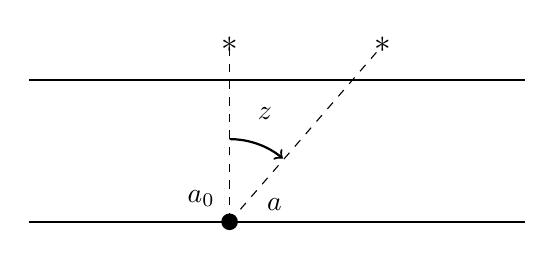
\begin{tikzpicture}[scale=1.5]
            % Draw two horizontal lines (horizon)
            \draw[thick] (-0.7,0) -- (3.5,0);
            \draw[thick] (-0.7,1.2) -- (3.5,1.2);

            % Observer's position (origin)
            \fill (1.0,0) circle (2pt);

            % Zenith direction (vertical dashed)
            \draw[dashed] (1.0,0) -- (1.0,1.5);

            % Star 1 (drawn as an asterisk)
            \node at (1.0,1.5) {\large $\ast$};
            % \node[above] at (1.0,1.55) {\small 1};

            % Star 2 (drawn as an asterisk)
            \node at (2.3,1.5) {\large $\ast$};
            % \node[above] at (2.3,1.55) {\small 2};

            % Zenith vector for star 2
            \draw[dashed] (1.0,0) -- (2.3,1.5);

            % z rotation between vertical and direction to star 2
            \draw[->, thick] (1.0,-0.2) ++(0,0.9) arc (90:50:0.7);
            \node at (1.3,0.92) {$z$};

            % Azimuth angles
            % \draw[->] (1.0,0) ++(-0.1,-0.2) arc (-120:0:0.22);
            \node at (0.76,0.2) {$a_0$};

            % \draw[->] (1.0,0) ++(0.2,-0.13) arc (-35:35:0.36);
            \node at (1.38,0.15) {$a$};
        \end{tikzpicture}
    % \end{figure}
    \end{minipage}

    \vspace{0.5em}

    Atmospheric extinction consists of both absorption and scattering by molecules and aerosols. 
    It increases with airmass and is typically parameterized using a linear relation in magnitudes:
    $$
        m(z) = m_0 + k a
    $$
    where $m(z)$ is the observed magnitude at zenith angle $z$, $m_0$ is the magnitude outside the atmosphere (zero airmass), $k$ is the extinction coefficient (which depends on wavelength and atmospheric conditions), and $a$ is the airmass, given by $a = 1/\cos(z)$. Alternatively, the airmass can also be expressed as $a = \alpha x$ for more precise geometric corrections, with $\alpha$ a proportionality constant and $x$ a path-length factor.

    \medskip

    An important process in atmospheric extinction is \textbf{Rayleigh scattering}: the scattering of light by small molecules. Rayleigh scattering is much stronger at shorter wavelengths (blue light), making the sky blue and causing stronger extinction for bluer astronomical sources.

    \medskip

    \item \textbf{Filter response} $F_\nu$: 
    
    Describes the transmission curve of the photometric filter, which determines how efficiently the filter transmits light at each frequency or wavelength. The effective bandpass and central wavelength are defined by this curve. 
    
    \vspace{0.5em}
    \begin{minipage}{0.62\textwidth}
    In practice, we often use the \textbf{effective (mean) wavelength}, defined as:
    $$
        \lambda_\mathrm{eq} = \frac{\int \lambda\,T_\lambda\,F_\lambda\,R_\lambda\, d\lambda}{\int T_\lambda\,F_\lambda\,R_\lambda\, d\lambda}
    $$
    where the integrals are performed over the bandpass and $T_\lambda$, $F_\lambda$, $R_\lambda$ are the atmospheric, filter, and detector response curves, respectively. The full width at half maximum (FWHM) is often used to characterize the width of the filter's transmission profile.
    \end{minipage}%
    \hfill
    \begin{minipage}{0.3\textwidth}
        \vspace{-2em}
        \begin{figure}[H]
            \centering
            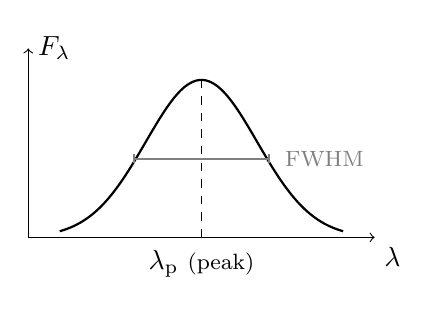
\begin{tikzpicture}[scale=2]
                % Axis
                \draw[->] (0,0) -- (2.2,0) node[below right] {$\lambda$};
                \draw[->] (0,0) -- (0,1.2) node[right] {$F_\lambda$};
        
                % Smooth filter transmission curve (Gaussian-like)
                \draw[thick,domain=0.2:2, samples=80, smooth] plot
                    (\x,{exp(-4*(\x-1.1)^2)}) ;
        
                % Dotted line at lambda_peak
                \draw[dashed] (1.1,0) -- (1.1,1) ;
                \node[below] at (1.1,-0.02) {$\lambda_\mathrm{p}$ \footnotesize (peak)};
        
                % FWHM line (half max = 0.5)
                \draw[gray,thick] (0.67,0.5) -- (1.53,0.5);
                \draw[gray,thick] (0.67,0.47) -- (0.67,0.53);
                \draw[gray,thick] (1.53,0.47) -- (1.53,0.53);
        
                % FWHM label
                \node[right,gray] at (1.57,0.5) {\footnotesize FWHM};
        
                % Annotate "lambda peak"
                % \node[below] at (1.1,-0.08) {\scriptsize $\lambda_\mathrm{p}$};
        
            \end{tikzpicture}
            \caption{Profile of a photometric filter response.}
        \end{figure}
    \end{minipage}

    \item \textbf{Telescope and detector response} $R_\nu$: 
    
    Represents the overall efficiency of the instrument, including the optics, mirrors, and detector (such as a CCD), and accounts for the quantum efficiency and reflective losses at each stage. Accurate knowledge of $R_\nu$ is essential for reliable photometry.

    \begin{itemize}
        \item \textbf{Photographic plates}: Early photographic plates had relatively poor photometric accuracy, with typical uncertainties around $\Delta m \approx 0.03$ mag.
        \item \textbf{CCD (Charge-Coupled Devices)}: Modern CCDs revolutionized photometry, offering uncertainties as low as $\Delta m \approx 0.001$ mag thanks to high quantum efficiency and linear response.
        \item \textbf{Photoelectric photometry}: Also widely used, providing precise measurements of incident flux using the photoelectric effect.
    \end{itemize}
\end{itemize}

\begin{observationblock}[K-correction]
    For galaxies at significant cosmological distances, one must apply a \textit{K-correction} to account for the fact that their observed light is redshifted due to cosmic expansion.
\end{observationblock}

\subsection{Absolute Magnitude}

The \textbf{absolute magnitude} $M$ of an astronomical object measures how bright it would appear if it were placed at a distance of 10 parsecs, removing the effects of distance to reflect its true luminosity.

More formally, the relationship between apparent magnitude $m$, absolute magnitude $M$, and distance $d$ (in parsecs) is governed by the distance modulus formula:
$$
m - M = -2.5 \log \left( \dfrac f F \right)
$$
Here, $f$ is the observed flux received from the source at an arbitrary distance $d$, and $F$ is the flux the same source would produce at exactly $10$ pc. Since flux decreases with the square of the distance, this relation naturally encodes the effects of distance on observed brightness.

\begin{minipage}{0.58\textwidth}
Knowing the relationship between flux and distance, we can derive the following relations:
\begin{align*}
    m - M &= 5 \log_{10}(d) - 5 \\[0.5em]
    m &= M + 5 \log_{10}(d) - 5 \\
    M &= m - 5 \log_{10}(d) + 5
\end{align*}

\vspace{0.3em}

The term $m - M$ is called the \bfit{distance modulus}. It provides a convenient tool for determining absolute magnitude when both apparent magnitude and distance are measured, and vice versa.
\end{minipage}%
\hfill
\begin{minipage}{0.4\textwidth}
\begin{figure}[H]
    \raggedright
    \includegraphics[width=0.9\textwidth]{assets/abs-mag.png}
    \vspace{-0.5em}
    \caption{\centering Absolute magnitude \cite{karttunen}}
\end{figure}
\end{minipage}

\begin{observationblock}[Absolute Magnitude of the Sun]
    The \textbf{absolute magnitude} of the Sun in the $V$ band is $M_{V\odot} = 4.83$. 

    The apparent $V$-band magnitude of the Sun as observed from Earth is $V_\odot = -26.74$. 
    The \textbf{distance modulus} for the Sun is:
    $$
        (V - M_V)_\odot = V_\odot - M_{V\odot} = -26.74 - 4.83 = -31.57
    $$
\end{observationblock}

\subsection{Color Index}

To measure stellar magnitudes with the highest precision, astronomers rely on photoelectric photometers, combined with carefully selected filters that restrict the incoming light to a specific wavelength range. The most widely adopted system is the \textit{Johnson photometric system}, which originally used three principal filters: $U$ (ultraviolet), $B$ (blue), and $V$ (visual).

The initial UBV system was later extended to the UBVRI, including $R$ (red) and $I$ (infrared). Each filter samples a distinct portion of the object's SED, so by comparing magnitudes measured through different filters, we gain direct information about a source's color and temperature.

\medskip

In any photometric system, the difference between two magnitudes measured in different passbands is called a \textbf{color index}. For example, the $B - V$ color index is defined as:
$$
B - V = m_B - m_V
$$
where $m_B$ and $m_V$ are the magnitudes measured through the $B$ and $V$ filters. 

More generally, the color index quantifies how the observed energy output changes between two wavelength intervals set by the respective filters. Formally, the $B - V$ color can be expressed as:
$$
B - V = C - 2.5 \log \left( \dfrac{\int_0^\infty d\lambda\, \delta_\lambda(B) f_\lambda}{\int_0^\infty d\lambda\, \delta_\lambda(V) f_\lambda} \right)
$$
where $\delta_\lambda(B)$ and $\delta_\lambda(V)$ are the response functions of the $B$ and $V$ filters, $f_\lambda$ is the spectral flux density, and $C$ is a system-dependent constant that ensures the correct photometric zero-point.

Importantly, the color index is independent of the source's distance:
$$
B - V = M_B - M_V + \cancel{5 \log d} - \cancel{5} - \cancel{5 \log d} + \cancel{5} = M_B - M_V
$$
where $M_B$ and $M_V$ are the absolute magnitudes in the $B$ and $V$ bands, respectively. The distance-dependent terms cancel, so the observed color index directly reflects intrinsic properties.

\medskip

Building upon this, the color index emerges as a fundamental tool for probing the physical properties of stars and galaxies, such as temperature, age and stellar population types.

\begin{figure}[H]
    \centering
    \begin{minipage}{0.6\textwidth}
        \centering
        \includegraphics[width=0.95\textwidth]{assets/col-idx.png}
    \end{minipage}%
    \hfill
    \begin{minipage}{0.39\textwidth}
        \vspace{0.5em}
        \captionof{figure}{Relative transmission profiles of filters used in the UBVRI magnitude system. The maxima of the bands are normalized to unity. The $R$ and $I$ bands are based on the system of Johnson, Cousins, and Glass, which includes also infrared bands $J$, $H$, $K$, $L$, and $M$. Previously used $R$ and $I$ bands differ considerably from these. \cite{karttunen}}
    \end{minipage}
\end{figure}

In particular, the $B-V$ color index serves as a straightforward and powerful temperature diagnostic for stars. Since hotter stars emit more radiation at shorter (bluer) wavelengths, they have lower (more negative) $B-V$ values; conversely, cooler stars appear redder and have higher $B-V$. The temperature corresponding to the color index is called \textbf{color temperature} $T_c$.

Color indices are also a useful diagnostic for broadly classifying the morphological types of galaxies. Elliptical galaxies typically exhibit redder colors, with $(B-V) \approx 1.5$, whereas spiral galaxies are generally bluer, around $(B-V) \approx 1.0$.

% According to the \textbf{Stefan-Boltzmann law}:
% $$
% L = 4\pi R^2 \sigma T_\mathrm{eff}^4
% $$
% where $L$ is the luminosity, $R$ is the radius and $T_\mathrm{eff}$ is the effective temperature.

\begin{tipsblock}[Practical use of color indices]
    In practical terms, color indices such as $U - B$ and $B - V$ are commonly reported, while the $V$ magnitude typically serves as the reference for absolute brightness.
\end{tipsblock}

\subsection{Magnitude corrections}

\subsubsection{Magnitude corrections for stars}

Interstellar dust and gas, collectively known as the 
Interstellar Medium (ISM), absorb and scatter starlight as 
it travels toward us. This process, called \textbf{interstellar extinction}, dims and reddens the observed 
light, causing the apparent magnitude $m$ to differ from 
the star's intrinsic magnitude $M$.

To correct for interstellar extinction, astronomers rely on \bfit{standard stars}: stars whose intrinsic magnitudes and colors are well known. By comparing the observed magnitudes of other stars to these calibrated standards, the effects of extinction can be accurately measured and removed.

To correct for extinction, we introduce the extinction term $A_\lambda$ at wavelength $\lambda$:

$$
M = m - 5 \log (d) + 5 - A_{\lambda}
$$

The value $A_{\lambda}$ quantifies the amount of extinction suffered by the light at wavelength $\lambda$. It is stronger at shorter wavelengths due to the wavelength dependence of the ISM opacity, meaning that blue light is affected more than red. Specifically, as we move from blue to infrared filters we have: $A_B > A_V > A_R > A_I$. This differential extinction alters the observed color index. For the $(B-V)$ color, the correction is:
$$
(B - V) = (B - V)_0 + \underbrace{A_B - A_V}_{E_{B-V} \neq 0}
$$
where $(B-V)_0$ is the intrinsic (unreddened) color index and $E_{B-V} = A_B - A_V$ is the \textbf{color excess}. The color excess encapsulates how much the ISM has reddened the starlight.



The relationship between extinction and color excess is characterized by the ratio
$$
R = \dfrac{A_V}{E_{B-V}} \approx 3
$$
for the diffuse Milky Way ISM. $R$ depends on properties, such as opacity, of the ISM along the line of sight. It is also related to the distance $d$ travelled through the ISM:
$$
A_V \propto d
$$

\begin{observationblock}[Colour as a distance tracer]
    By comparing a star's observed color to its intrinsic color $(B - V)_0$, if the stellar type is known, one can infer the color excess $E_{B-V}$, and thus estimate the extinction and, ultimately, the distance to the star.
\end{observationblock}

\subsubsection{Magnitude corrections for galaxies}

To accurately determine the intrinsic brightness of galaxies, astronomers must account for several corrections that affect the observed magnitude. The full correction formula is:

$$
M = m - 5 \log (d) + 5 - A_{\lambda} - A_{\lambda, i} - K + E
$$

where $A_{\lambda}$ is the MW extinction, $A_{\lambda, i}$ is the intrinsic extinction of the galaxy (due to its ISM), $K$ is the K-correction and $E$ is the evolution correction.

It is important to note that elliptical galaxies exhibit minimal extinction because they contain very little interstellar dust and gas. In contrast, spiral galaxies often display significant extinction, especially when observed \textit{"edge-on"} (when the disk of the galaxy is parallel to our line of sight) where starlight traverses a longer path through the galaxy's dusty disk.

\begin{itemize}
    \item \textbf{K-correction}:

    The \textbf{K-correction} adjusts for the fact that, due to redshift, a galaxy's observed spectrum is shifted and stretched to longer wavelengths compared to its rest-frame spectrum. This means an observed filter samples bluer rest-frame light. To compare intrinsic properties of galaxies at different redshifts, this effect must be corrected.
    Wavelengths are related by:
    $$
    \lambda_{\text{obs}} = \lambda_{\text{RF}} (1 + z)
    $$
    and thus, a filter of width $\Delta \lambda_{\text{obs}}$ corresponds to a narrower interval in the rest-frame:
    $$
    \Delta \lambda_{\text{RF}} = \frac{\Delta \lambda_{\text{obs}}}{1 + z}
    $$

    \vspace{-1.5em}

    \begin{figure}[H]
        \centering
        \begin{minipage}{0.42\textwidth}
            % Hand-drawn style schematic of the K-correction / SED shift
            \hspace{0.6em}
            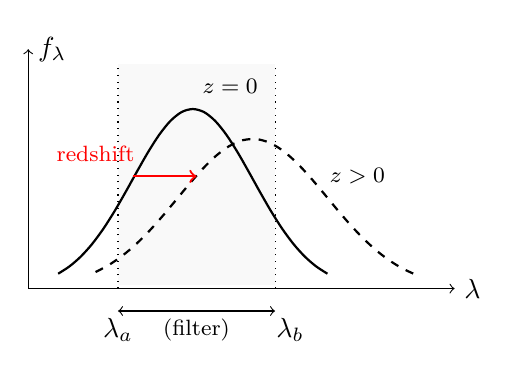
\begin{tikzpicture}[scale=0.95]
                % Axes
                \draw[->] (0.3,0) -- (6,0) node[right] {$\lambda$};
                \draw[->] (0.3,0) -- (0.3,3.2) node[right] {$f_\lambda$};

                % Vertical filter lines (lambda_a, lambda_b) and light gray fill
                \fill[gray!5] (1.5,0.05) rectangle (3.6,3.0);
                \draw[dotted] (1.5,0) -- (1.5,3.0);
                \draw[dotted] (3.6,0) -- (3.6,3.0);

                % Filter regions (lambda_a to lambda_b) -- shaded sections
                \draw[<->] (1.5,-0.3) -- (3.6,-0.3);
                \node at (1.5,-0.55) {$\lambda_a$};
                \node at (3.8,-0.55) {$\lambda_b$};
                \node at (2.55,-0.55) {\footnotesize (filter)};

                % SEDs
                % z = 0 SED
                \draw[thick] plot [smooth, domain=0.7:4.3] (\x, {2.4*exp(-((\x-2.5)^2)/1.3)});
                % label for z=0
                \node at (3,2.7) {\footnotesize $z=0$};

                % z > 0 SED (redshifted, dashed)
                \draw[thick, dashed] plot [smooth, domain=1.2:5.5] (\x, {2.0*exp(-((\x-3.3)^2)/2)});
                \node at (4.7,1.5) {\footnotesize $z > 0$};

                % Arrow showing redshift
                \draw[->, thick, red] (1.7,1.5) -- (2.55,1.5);
                \node[red] at (1.2,1.8) {\footnotesize {redshift}};
            \end{tikzpicture}
        \end{minipage}%
        \hfill
        \begin{minipage}{0.58\textwidth}
            \vspace{0.5em}
            \captionof{figure}{
                Effect of redshift on an observed galaxy spectrum: the rest-frame SED $z=0$ is not only shifted towards longer wavelengths at $z>0$ but also stretched (broadened) in wavelength. The features in the SED appear at longer wavelengths and are spread out due to the cosmological expansion. Thus, the fixed observed filter (between $\lambda_a$ and $\lambda_b$) samples different and broader parts of the SED as redshift increases.
            }
        \end{minipage}
    \end{figure}

    \vspace{-1em}

    \item \textbf{Evolution correction}: 

    The \textbf{evolution correction} ($E$) accounts for changes in a galaxy's stellar population and luminosity over time. As galaxies age, their stars evolve, altering overall brightness and color. Thus, a galaxy seen at higher redshift (when the Universe was younger) may look intrinsically brighter or bluer, not due to distance or observational effects.

    \begin{itemize}
    \item For \textbf{spiral galaxies}, we typically assume their star formation rate remains constant over time. The intrinsic properties of spirals change little, so the evolution correction is negligible: 
    $$
    E \approx 0
    $$

    \item In contrast, \textbf{elliptical galaxies} experienced most of their star formation in a brief, intense burst early in their history. Afterward, star formation largely ceased, and the stars passively age and redden. This causes their luminosity to fade significantly as the galaxy evolves. For these galaxies, the evolution correction can be substantial and is often parametrized as:
    $$
    E \sim K
    $$
    meaning that both evolutionary and K-corrections can be of similar magnitude and must be carefully accounted for when studying distant ellipticals.
    \end{itemize}

    \item \textbf{Extinction}:

    We have already discussed extinction in the context of stars, and the same principles apply to galaxies as well. If there is no material absorbing light along the line of sight, the relation between luminosity and distance is simply given by $L = \omega r^2 F$, where $L$ is the luminosity, $F$ is the observed flux, $\omega$ is a geometric factor, and $r$ is the distance to the source.

    However, when extinction occurs, the loss of light as it passes through the interstellar medium can be described by the equation
    $$
    dL = -\alpha L\, dr
    $$
    where the parameter $\alpha$, known as the \bfit{opacity}, quantifies how effectively the medium absorbs or blocks the radiation.The effect of extinction on observed luminosity is conveniently described by the \textbf{optical thickness} $\tau$, defined as:
    $$
    d\tau = \alpha\, dr
    $$

    The change in luminosity is then:
    $$
    dL = -L\, d\tau
    \qquad \Rightarrow \qquad
    \int_{L_0}^{L} \dfrac{dL'}{L'} = - \int_0^\tau d\tau'
    \qquad \Rightarrow \qquad
    L = L_0\, e^{-\tau}
    $$
    where $L_0$ is the intrinsic (unextinguished) luminosity.

    \vspace{-0.8em}

    \begin{figure}[H]
        \centering
        \includegraphics[width=0.9\textwidth]{assets/gal-ext.png}
        \vspace{-0.5em}
        \caption{Extinction effect on the observed flux of a galaxy. \cite{karttunen}}
    \end{figure}

    \vspace{-0.5em}

    The effect of extinction on luminosity and flux can be written explicitly as:
    $$
    L(r) = \omega r^2 F(r)
    $$
    where $L(r)$ is the luminosity at distance $r$, $\omega$ is a geometric factor, and $F(r)$ is the observed flux at $r$.
    Taking extinction into account, the observed flux becomes:
    $$
    F(r) = F_0 \, \frac{R^2}{r^2} \, e^{-\tau}
    $$
    where $F_0$ is the flux at a reference distance (or from a standard star), $R$ is the reference distance, and $\tau$ is the optical thickness (i.e., the total extinction along the line of sight).

    The distance modulus including extinction then becomes:
    $$
    m - M = -2.5 \log \left( \frac{F(r)}{F(10\,\mathrm{pc})} \right)
    $$
    Substituting the expression for $F(r)$ and $F(10\,\mathrm{pc})$, we obtain:
    $$
    m - M = 5 \log \left( \frac{r}{10\,\mathrm{pc}} \right) + \underbrace{2.5\, (\log e)\, \tau}_{A}
    $$
    where $A$ is the total extinction in magnitudes ($A = 1.086\,\tau$).

\end{itemize}

\subsection{Absolute Energy Distribution}